\documentclass[11pt, oneside]{article}   	% use "amsart" instead of "article" for AMSLaTeX format
\usepackage{geometry}                		% See geometry.pdf to learn the layout options. There are lots.
\geometry{letterpaper}                   		% ... or a4paper or a5paper or ... 
%\geometry{landscape}                		% Activate for rotated page geometry
%\usepackage[parfill]{parskip}    		% Activate to begin paragraphs with an empty line rather than an indent
\usepackage{graphicx}				% Use pdf, png, jpg, or eps§ with pdflatex; use eps in DVI mode
								% TeX will automatically convert eps --> pdf in pdflatex		
\usepackage{amssymb}

% % listings begin
\usepackage{listings}
% \providecommand{\GitRemote}{}
% \providecommand{\GitIdentifier}{master}
% \providecommand{\GitCheckout}[2][\GitIdentifier]{%
% % #1 being the version/branch
% % #2 being the file
% | \string"git archive --remote=\GitRemote #1 \detokenize{#2} 2>/dev/null | tar --extract --file - --to-stdout \string"%
% }
% % listings end

\usepackage{tikz}
\usetikzlibrary{positioning}
\usepackage{mathtools}

\usepackage{hyperref}
\usepackage{xcolor}
\definecolor{medium-blue}{rgb}{0,0,1}
\hypersetup{colorlinks, urlcolor={medium-blue}}

%SetFonts

%SetFonts

% External dependencies
\usepackage{pagecolor}
\input{../../../../include/hmath_descendant.tex}
% \input{https://github.com/hovey/include/blob/a9bf6db0394b5ba19e69653519a96c10eeb1e133/hmath_descendant.tex}
% https://tex.stackexchange.com/questions/500463/using-listinputlisting-to-include-a-specific-git-commit
% https://git-scm.com/docs/git-archive
% https://tex.stackexchange.com/questions/500463/using-listinputlisting-to-include-a-specific-git-commit

\title{Quadrilateral Quality}
\author{C.B.~Hovey}
%\date{}							% Activate to display a given date or n date

\begin{document}
\maketitle
%\section{}
%\subsection{}

% renewcommand{\GitRemote}{ssh://git@trac.sagemath.org/sage.git}
% \lstinputlisting{\GitCheckout{src/sage/coding/goppa.py}}
% \renewcommand{\GitRemote}{ssh://git@github.com:hovey/include.git}
% \lstinputlisting{\GitCheckout{hovey/include/hmath_descendant.tex}}

% \lstinputlisting{|\string"git archive --remote=ssh://git@server/repo.git VERSION path/to/file 2>/dev/null | tar --extract --file - --to-stdout\string"}
% \lstinputlisting{|\string"git archive --remote=ssh://git@github.com:hovey/include.git v0.0.1 hmath_descendant.tex 2>/dev/null | tar --extract --file hmath_descendant.tex --to-stdout\string"}
% \lstinputlisting{|\string"git archive --remote=https://git@github.com/hovey/include.git include/hmath_descendant.tex 2>/dev/null | tar --extract --file hmath_descendant.tex --to-stdout\string"}
% \lstinputlisting{|\string"git archive --remote=https://git@github.com/hovey/include.git v0.0.1 include/hmath_descendant.tex 2>/dev/null | tar --extract --file - --to-stdout\string"}


\begin{figure}[htb]
  \begin{center}

    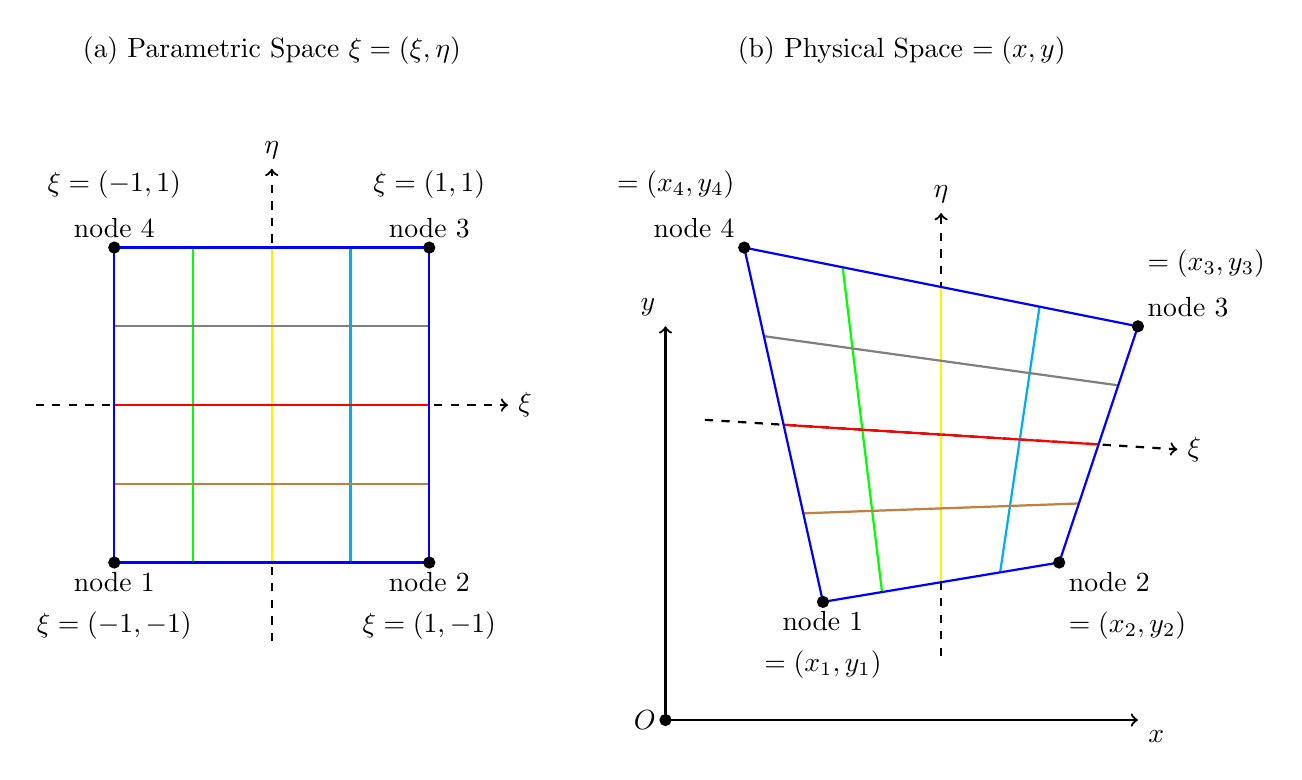
\begin{tikzpicture}
      % background grid
      % \draw[step=1cm,blue,dashed,very thin] (-9,0) grid (5,8);  % background grid
      % \foreach \x in {-9, -8, -6, -4, -2, 0, 2, 4, 5}
      %   \draw (\x cm,1pt) -- (\x cm,-1pt) node[anchor=north] {$\x$};
      % \foreach \y in {0, 2, 4, 6, 8}
      %   \draw (1pt,\y cm) -- (-1pt,\y cm) node[anchor=east] {$\y$};         
          
     % physical space
      %\node[draw,align=left] at (2,8.5) {(b) Physical Space}; % boxed
      \node[align=left] at (2,8.5) {(b) Physical Space $\vx = (x, y)$}; % unboxed
      % x-axis
      \draw[black,thick,->] (-1,0) -- (5,0) node[anchor=north west]{$x$};
      % y-axis
      \draw[black,thick,->] (-1,0) -- (-1,5) node[anchor=south east]{$y$};
      % origin
      \filldraw[black] (-1,0) circle (2pt) node[anchor=east]{$O$};


      % parametric space
      %\node[draw,align=left] at (-6,8.5) {(a) Parametric Space};  % boxed
      \node[align=left] at (-6,8.5) {(a) Parametric Space $\ve{\xi} = (\xi, \eta)$};  % unboxed
      % xi-axis
      \draw[black,thick,dashed,->] (-9,4) -- (-3,4) node[anchor=west]{$\xi$};
      % eta-axis
      \draw[black,thick,dashed,->] (-6,1) -- (-6,7) node[anchor=south]{$\eta$};

      % \draw[step=1cm,gray,very thin] (-8,2) grid (-4,6);  % grid
      % grid lines mapped from parameter space to physical space
      % center of grid is in figure space at (-6, 4)
      \draw[green, thick] (-7, 2) -- (-7, 6); % vertical grid 1
      \draw[yellow, thick] (-6, 2) -- (-6, 6); % vertical grid 2
      \draw[cyan, thick] (-5, 2) -- (-5, 6); % vertical grid 3
      \draw[brown, thick] (-8, 3) -- (-4, 3); % horizontal grid 1
      \draw[red, thick] (-8, 4) -- (-4, 4); % horizontal grid 2
      \draw[gray, thick] (-8, 5) -- (-4, 5); % horizontal grid 3

      % xi-axis mapped to physical space
      \draw[black,thick,dashed,->] (-0.5,3.8125) -- (5.5,3.4375) node[anchor=west]{$\xi$};
      % eta-axis mapped to physical space
      \draw[black,thick,dashed,->] (2.5,0.8125) -- (2.5,6.43775) node[anchor=south]{$\eta$};

      % grid lines mapped from parameter space to physical space
      \draw[green, thick] (1.75, 1.625) -- (1.25, 5.75); % vertical grid 1
      \draw[yellow, thick] (2.5, 1.75) -- (2.5, 5.5); % vertical grid 2
      \draw[cyan, thick] (3.25, 1.875) -- (3.75, 5.25); % vertical grid 3
      \draw[brown, thick] (0.75, 2.625) -- (4.25, 2.75); % horizontal grid 1
      \draw[red, thick] (0.5, 3.75) -- (4.5, 3.5); % horizontal grid 2
      \draw[gray, thick] (0.25, 4.875) -- (4.75, 4.25); % horizontal grid 3

      \draw[blue, thick] (-8,2) -- (-4,2);  % nodes 1-2
      \draw[blue, thick] (-4,2) -- (-4,6);  % nodes 2-3
      \draw[blue, thick] (-4,6) -- (-8,6);  % nodes 3-4
      \draw[blue, thick] (-8,6) -- (-8,2);  % nodes 4-1
      
      \filldraw[black] (-8,2) circle (2pt) node[anchor=north]{node $1$}; 
      \node[anchor=north] at (-8,1.5) {$\ve{\xi}= (-1, -1)$};  
      
      \filldraw[black] (-4,2) circle (2pt) node[anchor=north]{node $2$};  
      \node[anchor=north] at (-4,1.5) {$\ve{\xi}= (1, -1)$};  
      
      \filldraw[black] (-4,6) circle (2pt) node[anchor=south]{node $3$};
      \node[anchor=south] at (-4,6.5) {$\ve{\xi}= (1, 1)$};  

      \filldraw[black] (-8,6) circle (2pt) node[anchor=south]{node $4$};
      \node[anchor=south] at (-8,6.5) {$\ve{\xi}= (-1, 1)$};  
      
      \draw[blue, thick] (1,1.5) -- (4,2);  % nodes 1-2
      \draw[blue, thick] (4,2) -- (5,5);  % nodes 2-3
      \draw[blue, thick] (5,5) -- (0,6);  % nodes 3-4      
      \draw[blue, thick] (0,6) -- (1,1.5);  % nodes 4-1            
      
      \filldraw[black] (1,1.5) circle (2pt) node[anchor=north]{node $1$}; 
      \node[anchor=north] at (1,1) {$\vx = (x_1, y_1)$};  

      \filldraw[black] (4,2) circle (2pt) node[anchor=north west]{node $2$}; 
      \node[anchor=north west] at (4,1.5) {$\vx = (x_2, y_2)$};  

      \filldraw[black] (5,5) circle (2pt) node[anchor=south west]{node $3$}; 
      \node[anchor=south west] at (5,5.5) {$\vx = (x_3, y_3)$};  
      
      \filldraw[black] (0,6) circle (2pt) node[anchor=south east]{node $4$}; 
      \node[anchor=south east] at (0,6.5) {$\vx = (x_4, y_4)$};  

    \end{tikzpicture}

  \end{center}

  \caption{Parametric mapping $\vx = f(\ve{\xi})$ from parametric space to physical space.}
\label{fig:parametric_to_physical} % label must come after caption 
\end{figure}

\section{Isoparametric Mapping}
Let the parametric mapping $f: \ve{\xi} \mapsto \vx$ be defined as

\begin{align}
  x(\xi,\eta) & = \sum_{a=1}^4 N_a(\xi, \eta) \; x_a, \label{eq:shapex} \\
  y(\xi,\eta) & = \sum_{a=1}^4 N_a(\xi, \eta) \; y_a, \label{eq:shapey}
\end{align}
%\be
%x(\xi,\eta) = \sum_{a=1}^4 N_a(\xi, \eta) \; x_a, \mbox{ and }
%y(\xi,\eta) = \sum_{a=1}^4 N_a(\xi, \eta) \; y_a, 
%\ee
where a nodal {\bf shape function} is defined for each of the four nodes:
\begin{align}
  N_1(\xi, \eta) & \defe \tfrac{1}{4} (1 - \xi) (1 - \eta), \\
  N_2(\xi, \eta) & \defe \tfrac{1}{4} (1 + \xi) (1 - \eta), \\
  N_3(\xi, \eta) & \defe \tfrac{1}{4} (1 + \xi) (1 + \eta), \\
  N_4(\xi, \eta) & \defe \tfrac{1}{4} (1 - \xi) (1 + \eta).
\end{align}

\section{Jacobian}

For the quadrilateral element, the Jacobian $\vJ$ is calculated as 
the partial matrix of derivatives of $\vx = (x, y)$ with 
respect to $\ve{\xi} = (\xi, \eta)$, 
\be 
 \vJ(\xi, \eta) \defe 
 \left[
  \frac{\partial \vx}{\partial \ve{\xi}}
 \right]
 = 
 \left[
  \begin{tabular}{cc}
    $x,_{\tiny\xi}$ & $x,_{\tiny\eta}$ \\
    $y,_{\tiny\xi}$ & $y,_{\tiny\eta}$ 
  \end{tabular}
  \right].
\ee 
Substituting $x(\xi, \eta)$ and $y(\xi, \eta)$ with shape function equations
(\ref{eq:shapex})-(\ref{eq:shapey}) and expanding terms,  the Jacobian takes 
the form 
\be 
 \vJ(\xi, \eta) = \frac{1}{4} 
 \left[
  \begin{tabular}{rrrr}
    $-1 + \eta$ & $1 - \eta$ & $1 + \eta$ & $-1 - \eta$ \\
    $-1 + \xi$ & $-1 - \xi$ & $1 + \xi$ & $1 - \xi$ 
  \end{tabular}
  \right]
  \left[ 
  \begin{tabular}{cc}
    $x_1$ & $y_1$ \\
    $x_2$ & $y_2$ \\
    $x_3$ & $y_3$ \\
    $x_4$ & $y_4$ \\
  \end{tabular}
  \right].
\ee 
The determinant of the Jacobian, $\det(\vJ)$, can be found to be 
\be 
\det(\vJ\left(\xi, \eta)\right) = c_0 + c_1 \xi + c_2 \eta,
\ee 
where
\begin{align}
  c_0 & = \frac{1}{8} \left[(x_1 - x_3) (y_2 - y_4) - (x_2 - x_4) (y_1 - y_3) \right], \\
  c_1 & = \frac{1}{8} \left[(x_3 - x_4) (y_1 - y_2) - (x_1 - x_2) (y_3 - y_4) \right], \\
  c_2 & = \frac{1}{8} \left[(x_2 - x_3) (y_1 - y_4) - (x_1 - x_4) (y_2 - y_3) \right].
\end{align}

\section{Quality}

Important {\em Metrics for Quadrilateral Elements}\footnote{See \href{https://cubit.sandia.gov/files/cubit/16.04/help_manual/WebHelp/cubithelp.htm}{Cubit} or \href{https://coreform.com/cubit_help/mesh_generation/mesh_quality_assessment/quadrilateral_metrics.htm}{Coreform}.} follow:

\begin{itemize}
    \item Aspect ratio: Maximum edge length ratios at the quadrilateral center.  Citation: Robinson 1987.\footnote{Robinson J. CRE method of element testing and the Jacobian shape parameters. Engineering Computations. 1987 Feb 1.}
  \item Jacobian metric: Minimum pointwise volume of local map at the four corners and center of quadrilateral.  Dimension: $L^2$.  Full range: $(-\infty, \infty)$.  Acceptable range: None.  Citation: Knupp 2000.\footnote{Knupp PM. Achieving finite element mesh quality via optimization of the Jacobian matrix norm and associated quantities. Part II—a framework for volume mesh optimization and the condition number of the Jacobian matrix. International Journal for numerical methods in engineering. 2000 Jul 20;48(8):1165-85. OSTI \href{link}{https://www.osti.gov/servlets/purl/5009}.}
  \item Scaled Jacobian metric: For a linear element, the minimum Jacobian [at a point] divided by the lengths of the two edge vectors [connecting to that point].  Dimension: $L^0$.  Full range: $[-1.0, 1.0]$.  Acceptable range $[0.5, 1.0]$.  Citation: Knupp 2000, {\em op.~cit.}.
\end{itemize}

Following {\em The Verdict Geometry Quality 
Library} documentation,\footnote{Knupp PM, Ernst CD, Thompson DC, Stimpson CJ, Pebay PP. The verdict geometric quality library. Sandia National Laboratories (SNL), Albuquerque, NM, and Livermore, CA (United States); 2006 Mar 1.  OSTI \href{link}{https://www.osti.gov/servlets/purl/901967}.} we compute the minimum Jacobian as the minimum of the four Jacobians computed at each vertex:\footnote{Knupp 2006, {\em op.~cit.}~at 42.}
\be 
J_{\min} \defe \min(J_1, J_2, J_3, J_4),
\ee 
and the minimum scaled Jacobian as the minimum of the four Jacobians computed at 
each vertex divided lengths of the two element edges connected 
to that vertex\footnote{Knupp 2006, {\em op.~cit.}~at 51.}
\be 
\hat{J}_{\min} \defe \min\left(\frac{J_1}{e_4 e_1}, \frac{J_2}{e_1 e_2}, 
\frac{J_3}{e_2 e_3}, \frac{J_4}{e_3 e_4}\right),
\ee 
where the following edge lengths are defined:
\begin{align}
e_1 &\defe \; \norm{\vx_2 - \vx_1}, \\
e_2 &\defe \; \norm{\vx_3 - \vx_2}, \\
e_3 &\defe \; \norm{\vx_4 - \vx_3}, \\
e_4 &\defe \; \norm{\vx_1 - \vx_4}.
\end{align}

\end{document}

